% SPDX-FileCopyrightText: Copyright (c) 2023-2025 Yegor Bugayenko
% SPDX-License-Identifier: MIT

\documentclass{article}
\usepackage{../lecture-notes/notes}
\usepackage{amsmath}
\usepackage{relsize}
\newcommand*\thetitle{Dead Code}
\begin{document}

\lnTitlePage{12}{24}{zN0gX9m6a2k}

\pptBanner{Motivating Example}
\begin{multicols}{2}
Before (\textcolor{red}{wrong}):\par
{\small\begin{ffcode}
class Book
  private int id;
  public Book(int i)
    this.id = i;
  public int getId()
    return this.id;

  (*@\textcolor{red}{private int setId(int i)}@*)
    (*@\textcolor{red}{this.id = i;@*)
\end{ffcode}
}
\par\columnbreak\par
After (\textcolor{green}{better}):\par
{\small\begin{ffcode}
class Book
  private final int id;
  public Book(int i)
    this.id = i;
  public int getId()
    return this.id;
\end{ffcode}
}
\end{multicols}
\plush{}

\pptBanner{Dead Code Elimination (Compiler Optimization)}
\begin{multicols}{2}
Dead code is here:\par
{\small\begin{ffcode}
void main(int x) {
  int a = 42;
  if (x > 0) {
    (*@\textcolor{red}{a = 256;}@*)
  }
  a = 7;
  print(a);
}
\end{ffcode}
}
\par\columnbreak\par
``Dead code refers to computations whose \ul{results are never used}. Code that is dead can be eliminated without affecting the behavior of the program.''\par
{\scriptsize Source: \textit{Compiler Techniques for Code Compaction}, Saumya K. Debray, William Evans, Robert Muth, Bjorn De Sutter, ACM Transactions on Programming languages and Systems (TOPLAS), 22(2), 2000 \par}
\end{multicols}
\plush{}

\lnQuote
  [Mika M\"{a}ntyl\"{a}]
  {mika-mantyla}
  {Dead code is code that has been used in the past, but is currently never executed. Dead code \ul{hinders} code \ul{comprehension} and makes the current program structure \ul{less obvious}.}
  {mantyla2003}

\lnQuote
  [Sebastian Eder]
  {sebastian-eder}
  {We conducted the study on the level of methods in the sense of object oriented programming. The systems contains 25,390 methods. We found that \ul{25\% of all methods} were never used during the complete period.}
  {eder2012}

\lnPitch{
  \pptBanner{Unreachable/Dead Methods in Java}
  \pptPic{.9}{unreachable.png}\par
  \lnSource{romano2016graph}}

\lnQuote
  [Simone Romano]
  {simone-romano}
  {Although there is some consensus on the fact that dead code is a common phenomenon, it could be \ul{harmful}, and it seems to matter to software professionals; surprisingly, dead code has received very little empirical attention from the software engineering research community.}
  {romano2018}

\lnPitch{
  \begin{multicols}{2}
  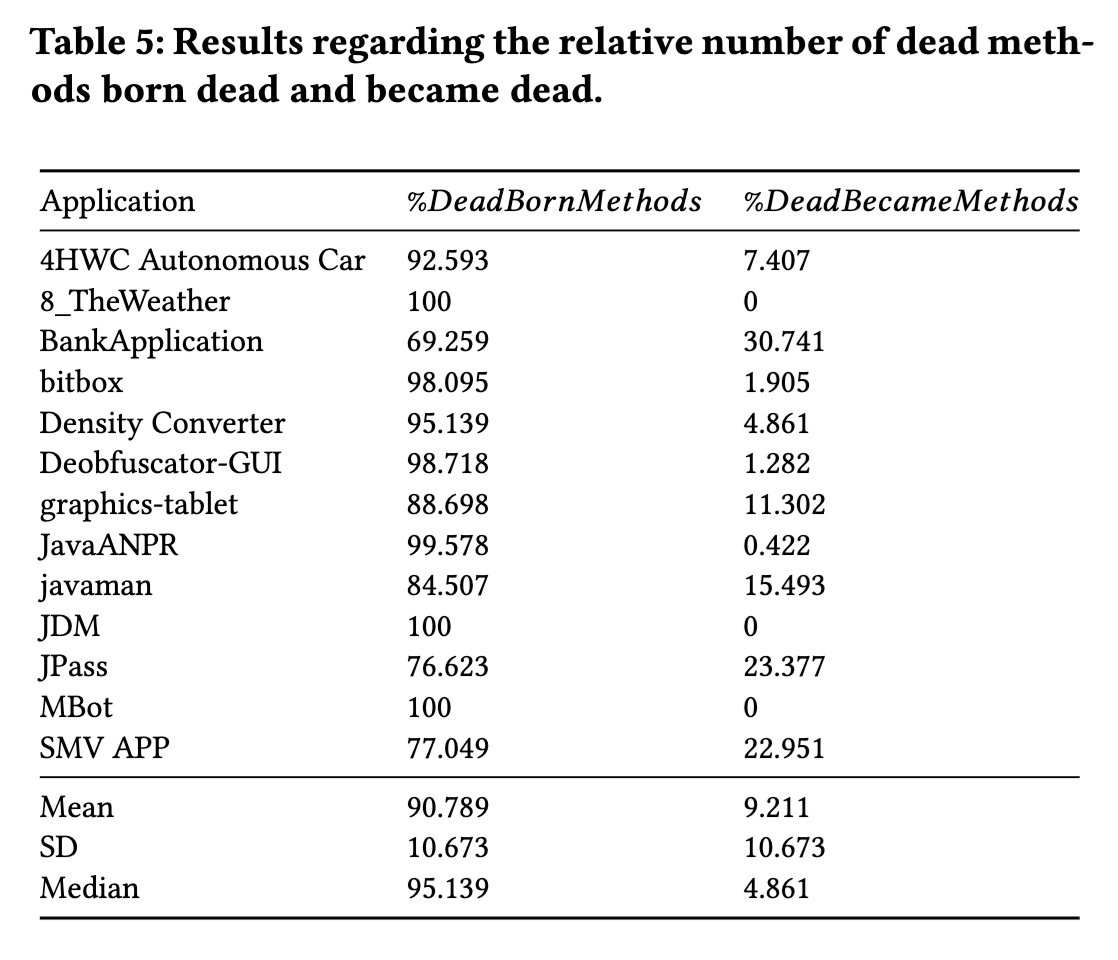
\includegraphics[width=\linewidth]{born-dead.png}
  \par\columnbreak\par
  ``\begin{inparaenum}[i)]\item ...; \item dead methods generally \ul{survive} for a long time, in terms of commits, before being buried or revived; \item dead methods are \ul{rarely revived}; and \item most dead methods are dead \ul{since the creation} of the corresponding methods.\end{inparaenum}''
  \lnSource{caivano2021exploratory}
  \end{multicols}}

\lnPitch{
  \begin{multicols}{2}
  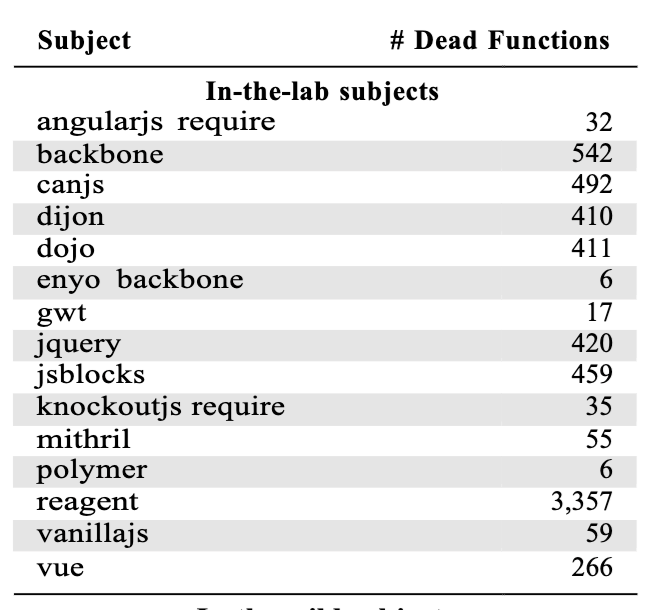
\includegraphics[width=\linewidth]{js-deads.png}
  \par\columnbreak\par
  ``The elimination of JavaScript dead code leads to noticeable (and statistically significant) differences in terms of the number of performed HTTP requests only for in-the-lab subjects.''
  \lnSource{malavolta2023javascript}
  \end{multicols}}

\lnQuote
  [Katriel Cohn-Gordon]
  {katriel-cohn-gordon}
  {At \textcolor{orange}{Meta}, in the last year alone, we removed petabytes of data across 12.8 million distinct assets, and deleted over 104 million lines of code.}
  {shackleton2023dead}

\lnQuote
  [Pietro Cassieri]
  {pietro-cassieri}
  {The results indicate that, after removing dead methods, the \ul{internal structure} of the source code significantly \ul{improves}, while the \ul{space} to store executable code significantly decreases along with the time to compile source code.}
  {romano2024folklore}

\lnPitch{
  \pptBanner{Volatility Metric}
  \begin{multicols}{2}
  \scalebox{.7}{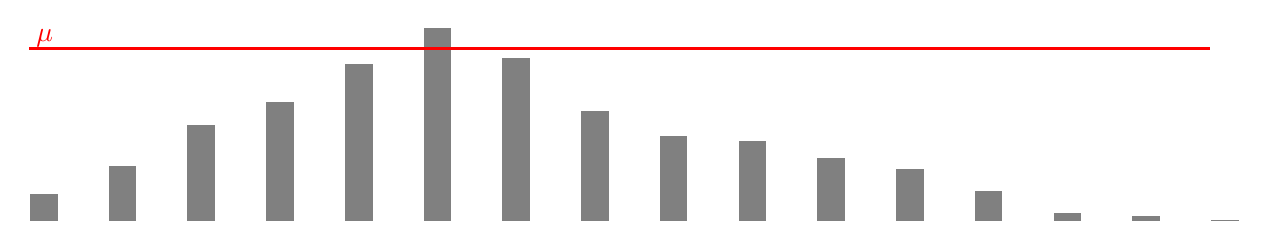
\begin{tikzpicture}[every node/.style={rectangle, minimum width=1em, fill=gray, anchor=south west, font={\color{white}}, inner sep=0pt}]
  \node[minimum height=1em] at (0,0) {};
  \node[minimum height=2em] at (1,0) {};
  \node[minimum height=3.5em] at (2,0) {};
  \node[minimum height=4.3em] at (3,0) {};
  \node[minimum height=5.7em] at (4,0) {};
  \node[minimum height=7em] at (5,0) {};
  \node[minimum height=5.9em] at (6,0) {};
  \node[minimum height=4em] at (7,0) {};
  \node[minimum height=3.1em] at (8,0) {};
  \node[minimum height=2.9em] at (9,0) {};
  \node[minimum height=2.3em] at (10,0) {};
  \node[minimum height=1.9em] at (11,0) {};
  \node[minimum height=1.1em] at (12,0) {};
  \node[minimum height=0.3em] at (13,0) {};
  \node[minimum height=0.2em] at (14,0) {};
  \node[minimum height=0.05em] at (15,0) {};
  \draw[color=red, very thick] (0,2.2) node[fill=none] {\(\mu\)} -- (15,2.2);
  \end{tikzpicture}}
  \par
  ``The variance \(\text{Var}(g)\) is the \textbf{Volatility} of the source code.
  The smaller the Volatility the more \textit{cohesive} is the repository
  and the smaller the amount of the abandoned code inside it.''
  \par\columnbreak\par
  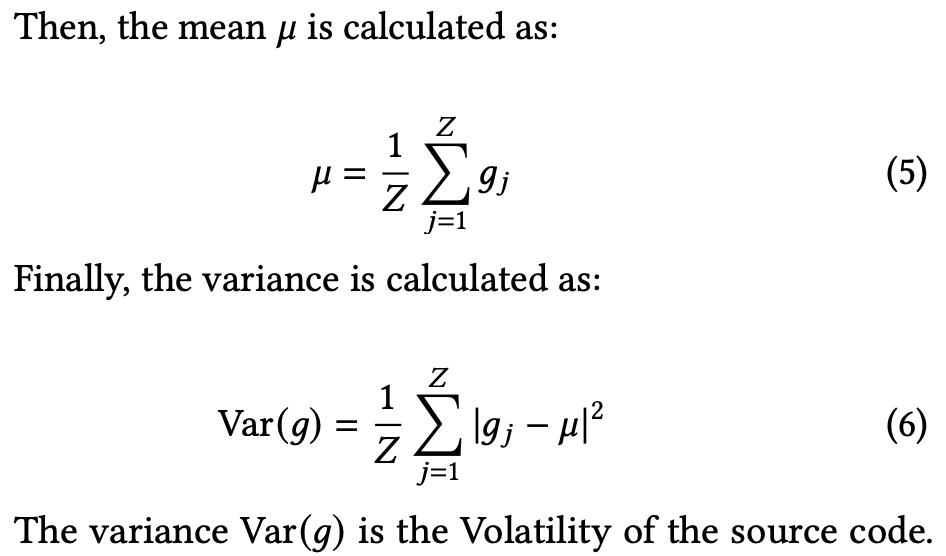
\includegraphics[width=.95\columnwidth]{formula.png}
  \lnSource{bugayenko2021volatility}
  \end{multicols}}

\lnPitch{
  \pptBanner{Volatility vs. Number of Files in a Repo}
  \pptPic{.5}{graph.png}
  \lnSource{bugayenko2021volatility}}

\lnQuote
  [Ciera Jaspan]
  {ciera-jaspan}
  {Our survey results show that engineers at Google strongly prefer our monolithic repo, and that \ul{visibility} of the codebase and simple \ul{dependency management} were the primary factors for this preference.}
  {jaspan2018advantages}

\lnPitch{\pptBanner{Monolithic Repositories}
  {\small\begin{description}
  \item[Centralization]
    {\scriptsize The codebase is contained in a single repo encompassing multiple projects.}
  \item[Visibility]
    {\scriptsize Code is viewable and searchable by all engineers in the organization.}
  \item[Synchronization:]
    {\scriptsize The development process is trunk-based; engineers commit to the head of the repo.}
  \item[Completeness]
    {\scriptsize Any project in the repo can be built only from dependencies also checked into the repo.
    Dependencies are unversioned; projects must use whatever version of their dependency is at the repo head.}
  \item[Standardization]
    {\scriptsize A shared set of tooling governs how engineers interact with the code, including building, testing, browsing, and reviewing code.}
  \end{description}}\par
  \lnSource{jaspan2018advantages}}

\lnQuote
  [James Whittaker]
  {james-whittaker}
  {Most code at Google shares a \ul{single} repository and common tool chain. This single repository makes a great deal of sense as engineers moving from project to project have little to \ul{relearn}.}
  {whittaker2012google}

\lnQuote
  [John Penix]
  {john-penix}
  {Software development at Google happens quickly and at scale. The Google codebase receives over \ul{20 changes per minute} and 50 percent of the files change every month!}
  {whittaker2012google}

\lnQuote
  [Durham Goode]
  {durham-goode}
  {\textcolor{orange}{Facebook}'s main source repository is enormous---many times larger than even the Linux kernel, which checked in at \ul{17 million lines of code} and \ul{44,000 files} in 2013.}
  {goode2014}

\lnQuote
  [Rachel Potvin]
  {rachel-potvin}
  {The \textcolor{orange}{Google} codebase includes approximately \ul{one billion files} and has a history of approximately 35 million commits spanning Google's entire 18-year existence. The repository contains \ul{86TBa} of data, including approximately \ul{two billion lines of code} in nine million unique source files.}
  {potvin2016}

\lnQuote
  [Tomas Votruba]
  {tomas-votruba}
  {Before monorepo, I had to upgrade every package manually, which resulted in dissonance: one package used Symfony\textbackslash{}Console 3.2, but other only 2.8 and it got messy \ul{for no reason}.}
  {votruba2017}

\lnPitch{
  \pptBanner{What About Yandex?}
  \pptPic{.8}{yandex-repo.png}
  \lnSource{kruglov2018yandex}}

\lnPitch{\pptBanner{Benefits of ``Manyrepo'' Approach}
  {\small\begin{description}
  \item[Encapsulation]
    Each repo encapsulates and hides its details from everybody else.
  \item[Fast Builds]
    When a repo is small, the time its automated build takes is small.
  \item[Accurate Metrics]
    Calculating LoC for a large repository doesn't make any sense.
  \item[Homogeneous Tasks]
    It's easier to make tasks similar in size and complexity.
  \item[Single Coding Standard]
    Smaller repositories look more beautiful.
  \item[Short Names]
    Smaller namespaces mean better maintainability.
  \item[Simple Tests]
    More dependencies are difficult to mock and test.
  \end{description}}\par
  \lnSource{bugayenko2018blog0905}}

\end{document}
